\documentclass[10pt]{article}
\usepackage[a4paper, left=1.5cm, right=1.5cm, top=3.5cm]{geometry}
%\usepackage[german]{babel}
\usepackage[]{graphicx}
\usepackage[]{multicol}
\usepackage[]{titlesec}
\usepackage[]{wrapfig}
\usepackage[]{blindtext}
\usepackage[]{lipsum}
\usepackage[]{caption}
\usepackage[]{listings}
\usepackage[]{fancyhdr}
\usepackage[]{nopageno}
\usepackage[]{authblk}
\graphicspath{{images/}}
\fancyhf[]{}

% own fig. env. for multicols
\newenvironment{Figure}
  {\par\medskip\noindent\minipage{\linewidth}}
  {\endminipage\par\medskip}

\begin{titlepage}
    \title{Computerphysik -- Abgabe 1}
    \author[1]{Michael J. P. Vogt\thanks{481204012, jdksljf, m.vogt@uni-bonn.de}}
    \author[1]{Angelo V. Brade\thanks{50035421, s72abrad, a.brade@uni-bonn.de}}
    \affil[1]{Rhenish Friedrich Wilhelm University of Bonn}
    \date{\today}
\end{titlepage}
%\let\runauthor\@author

\begin{document}
\pagenumbering{gobble}
\maketitle
\newpage

\tableofcontents
\newpage

\pagenumbering{arabic}

\pagestyle{fancy}
\fancyhead[R]{\thepage}
\fancyhead[L]{\leftmark}

\begin{multicols}{2}
[
    \section{Abstract}
    Hier ein Abstract.
]
\subsection{The standard Lorem Ipsum passage, used since the 1500s}
\lipsum[1]

\lipsum[6]

\subsection{Section 1.10.32 of "de Finibus Bonorum et Malorum", written by Cicero in 45 BC}
\lipsum[2]
\begin{Figure}
    \centering
    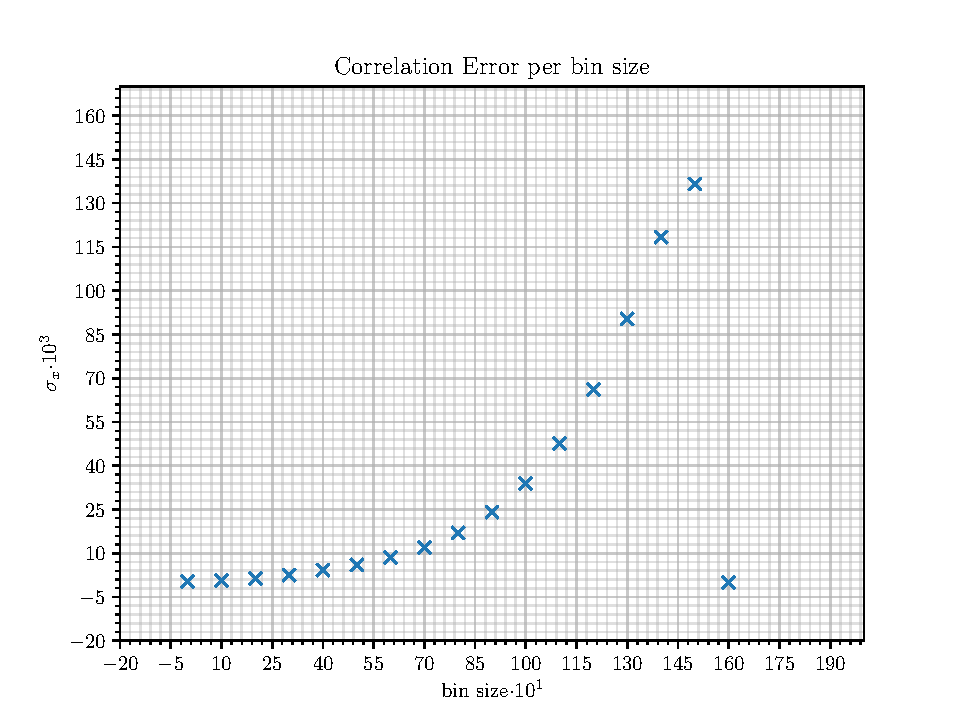
\includegraphics[width=1.0\linewidth]{CorrelationErrorPerBinSize}
    \captionof{figure}{Correlation Function}
\end{Figure}
\lipsum[3]

\subsection{1914 translation by H. Rackham}
\lipsum[4]
\(\sum_{i}^{N}a_i\)
\[\sum_{i}^{N}a_i\]
\begin{equation}
\sum_{i}^{N}a_i
\end{equation}

\subsection{Section 1.10.33 of "de Finibus Bonorum et Malorum", written by Cicero in 45 BC}
\lipsum[5]


\end{multicols}

\end{document}